\documentclass[10pt]{beamer}

\usetheme[progressbar=frametitle]{metropolis}
\usepackage{appendixnumberbeamer}
\usepackage{amsmath}
\usepackage{algorithmicx}
\usepackage{algpseudocode}

\usepackage{booktabs}
\usepackage[scale=2]{ccicons}
\usepackage{pgfpages}
\usepackage{hyperref}


\usepackage{pgfplots}
\usepgfplotslibrary{dateplot}
\pgfplotsset{compat=1.11}

\usepackage{xspace}
%%\setbeameroption{show notes on second screen=right} 
%\setbeamertemplate{note page}{\pagecolor{yellow!5}\insertnote}

\pgfdeclareimage[width=\paperwidth]{mybackground}{src/futureits.png}
\defbeamertemplate{description item}{align left}{\insertdescriptionitem\hfill}

\newcommand{\themename}{\textbf{\textsc{metropolis}}\xspace}
\hypersetup{pdfpagemode=FullScreen}




\title{Adaptive Beamforming for future ITS}
\subtitle{A neural network approach to antenna beam steering for mmWave Systems}
\author{Clifford Beta \and \\Anne Okemwa}
 \date{\today}

 \titlegraphic{\hfill
\includegraphics[height=1.5cm]{src/logo.png}}

\begin{document}

\maketitle
    
\begin{frame}{mmWave Communication Potential}
  \begin{itemize}[<+- | alert@+>]
    \item \huge multi-gigabit-per second communication
    \item \huge very low latency
  \end{itemize}
\end{frame}
{
\usebackgroundtemplate{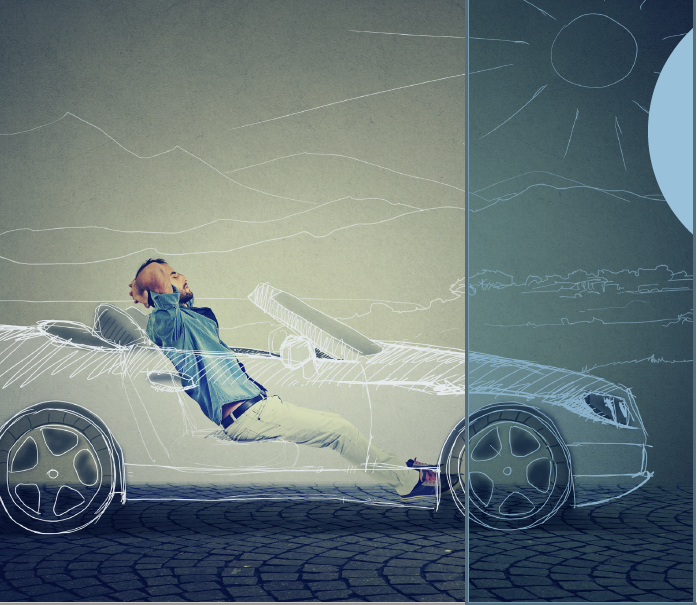
\includegraphics[width=\paperwidth]{src/autonomous.png}}
\begin{frame}{Applications}
  \begin{itemize}[<+- | alert@+>]
    \item \huge Autonomous driving
    \item \huge Immersive gaming
    \item \huge Virtual reality
    \item \huge Augmented reality
  \end{itemize}
\end{frame}
}
\begin{frame}{Problem}
	\begin{columns}
    \begin{column}{.45\textwidth}
    \vfill
        \begin{overlayarea}{\textwidth}{.45\textheight}
 		 \only<1-|handout:0>{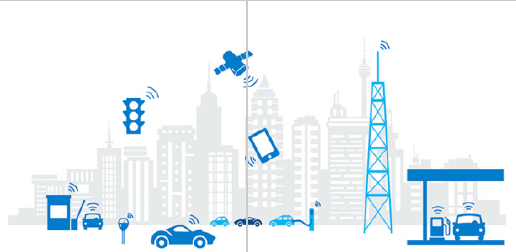
\includegraphics[width=4cm]{src/futureits.png}}
		\end{overlayarea}%
    \end{column}
    \begin{column}{.45\textwidth}
    \begin{overlayarea}{\textwidth}{.45\textheight}
 		\only<2>{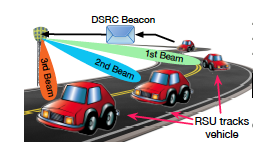
\includegraphics[width=4cm]{src/vehiclemobility.png} }
		\end{overlayarea}%
    \end{column}
\end{columns}
	\begin{columns}
	
    \begin{column}{.45\textwidth}
    \begin{itemize}
          \item Increased vehicular mobility \pause
          \end{itemize}
    \end{column}
    \begin{column}{.45\textwidth}
    \begin{itemize}
  \item Need for constant beam realignment. 
  \end{itemize}
    \end{column}
    \end{columns}
\end{frame}

{
\usebackgroundtemplate{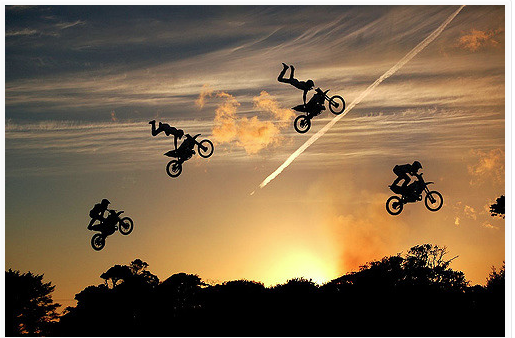
\includegraphics[width=\paperwidth]{src/sequence.png}}
\begin{frame}[fragile]{Model}
 \par
\end{frame}
}

\begin{frame}[fragile]{Neural Network}
  Neural networks have been proven to have the ability to compute any function, even

  \begin{verbatim}   {Sequence prediction problems}\end{verbatim}

  at which \emph{LSTMs} shine \ldots
\end{frame}

\begin{frame}[fragile]{tanh Neuron}
\begin{columns}
    \begin{column}{.3\textwidth}
       \begin{equation*}   
  		 \sigma (z) \equiv  \tanh(z)
 		 \end{equation*}
    \end{column}
    \begin{column}{.6\textwidth}

		 \begin{figure}
      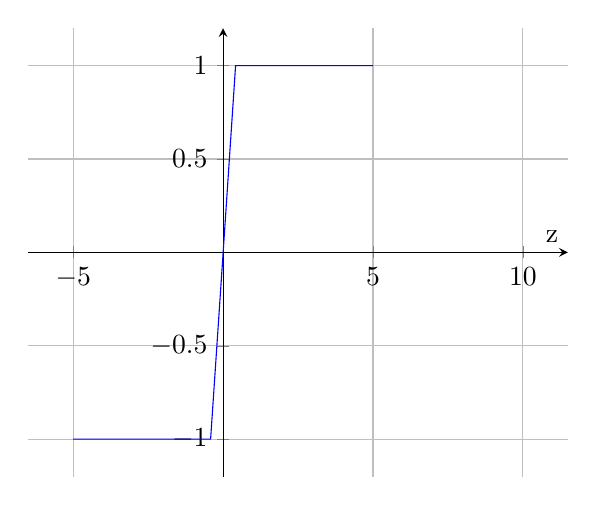
\begin{tikzpicture}
\begin{axis}[grid=both,
          xmax=10,ymax=1,
          axis lines=middle,
          xlabel = z,
          restrict y to domain=-7:12,
          enlargelimits]
\addplot[blue]  {tanh(deg(x))};
\end{axis}
\end{tikzpicture}
\end{figure}

	  \end{column}
\end{columns}

\end{frame}

\begin{frame}{ReLU Neuron}
\begin{columns}
    \begin{column}{.3\textwidth}
        \begin{equation*}   
  		 \sigma (z) \equiv  max(0,z)
 		 \end{equation*}
    \end{column}
    \begin{column}{.6\textwidth}
    \begin{figure}
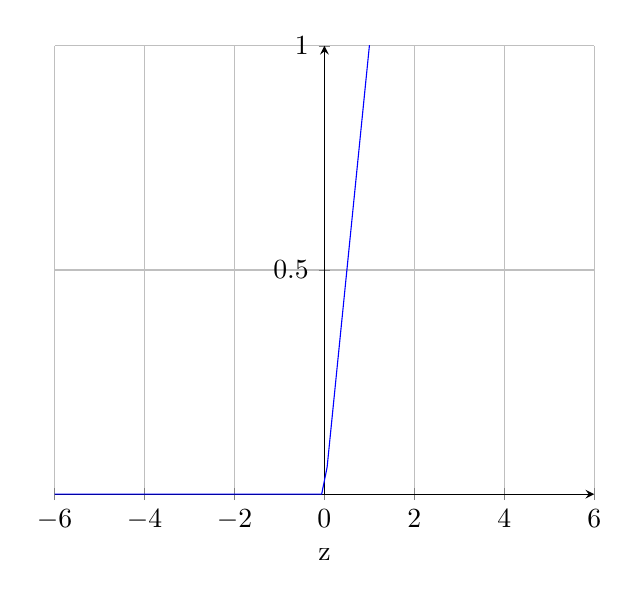
\begin{tikzpicture}
    \begin{axis}%
    [
        grid=major,     
        xmin=-6,
        xmax=6,
         xlabel = z,
        axis x line=bottom,
        ytick={0,.5,1},
        ymax=1,
        axis y line=middle,
    ]
        \addplot%
        [
            blue,%
            mark=none,
            samples=100,
            domain=-6:6,
        ]
        (x,{max(0,x)});
    \end{axis}
\end{tikzpicture}
  \end{figure}
    \end{column}
\end{columns}


\end{frame}

\begin{frame}{Sigmoid Neuron}
\begin{columns}
    \begin{column}{.3\textwidth}
        \begin{equation*}   
  		 \sigma (z) \equiv  \frac{1}{1+ e^ {-z}}
 		 \end{equation*}
    \end{column}
    \begin{column}{.6\textwidth}
    \begin{figure}
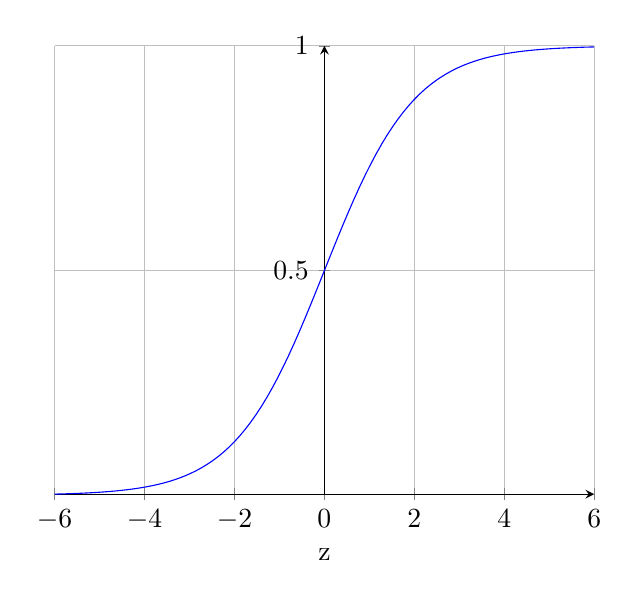
\begin{tikzpicture}
    \begin{axis}%
    [
        grid=major,     
        xmin=-6,
        xmax=6,
         xlabel = z,
        axis x line=bottom,
        ytick={0,.5,1},
        ymax=1,
        axis y line=middle,
    ]
        \addplot%
        [
            blue,%
            mark=none,
            samples=100,
            domain=-6:6,
        ]
        (x,{1/(1+exp(-x))});
    \end{axis}
\end{tikzpicture}
  \end{figure}
    \end{column}
\end{columns}
\end{frame}
\begin{frame}{LSTM}
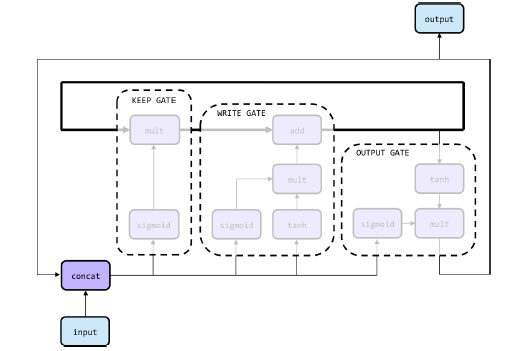
\includegraphics[width=\textwidth]{src/lstm.png} 
\end{frame}

\begin{frame}{Neural Network}
\begin{columns}
\begin{column}{.4\textwidth}
\begin{itemize}[<+- | alert@+>]
    \item  Feed forward Neural Networks
    \item  Recurrent Neural Networks 
    \begin{itemize}
    \item Long short term memory RNN (LSTM)
    \end{itemize}
  \end{itemize}
  \end{column}
    \begin{column}{.5\textwidth}
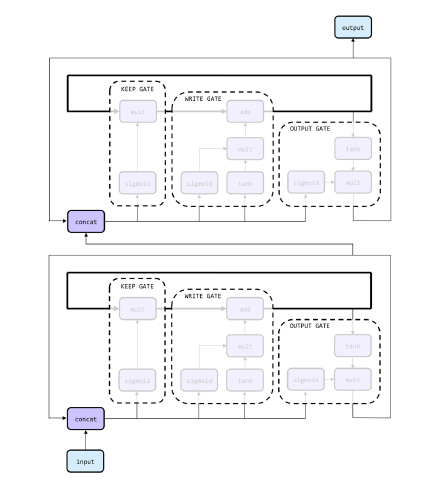
\includegraphics[width=\textwidth]{src/lstmnet.png} 
\end{column}
  \end{columns}
\end{frame}
\begin{frame}{Beam-forming}
	\begin{itemize}
	\item Least Mean Squares (LMS)
	\item Sample Matrix Inversion (SMI)
	\item Recursive Least Squares (RLS)
	\item Conjugate Gradient Method (CGM)
	\end{itemize}
\end{frame}
\begin{frame}{Algorithm}
\begin{algorithmic}
\Require Vehicles encapsulate position, motion and velocity in beacons
\Ensure Serving node has not changed after every update interval.
\If {New beacon received } 
\\Find Closest node 
\If {$Received position \neq Predicted position $}
 \\Beamforming: Align beam based on received position
\Else
\\Predict current position of vehicle \\
 Beamforming: Align beam based on predicted position
 \EndIf
\EndIf
\end{algorithmic}
\end{frame}

\begin{frame}{Merits}
	\begin{description}
		\item [Higher SNR] 
		%The highly directional transmission improves the link budget, this increasing the range, both open-space and for indoor penetration
		\item [Interference avoidance and rejection] 
		%Beamforming overcomes external and internal (CCI) interference by exploiting the spatial properties of the antennas. Since the interference comes from a certain direction, the beamformer can apply a nulling technique ? send a ?null? towards the interferer, canceling it out.
		\item [Higher network efficiency] 
		%By significantly reducing the CCI, beamforming can allow much denser deployments than single antenna systems. Thanks to higher link budget, the likelihood of running high-order modulations (64QAM, 16QAM) is much higher even at the edges of the cell. Overall capacity is greatly improved.
	\end{description}
\end{frame}

\begin{frame}{Technologies}
	\begin{description}
		\item [Tensorflow]  Google's open source deep learning framework for motion prediction
		\item [Matlab] for antenna simulations
		\item [DSRC] Dedicated Short Range Communication
	\end{description}
\end{frame}

{\setbeamercolor{palette primary}{fg=black, bg=yellow}
\begin{frame}[standout]
  Questions?
\end{frame}
}

\begin{frame}[standout]
  \url{https://github.com/Clifford-Beta/adaptive-beamforming}
\end{frame}
\end{document}
